\documentclass[letter,11pt]{article}
%\documentclass[letter,twoside,11pt]{article}

\usepackage[spanish,es-nodecimaldot]{babel}
\usepackage[utf8]{inputenc}

\usepackage{lmodern}
\usepackage[T1]{fontenc}
\usepackage{textcomp}

\usepackage{graphicx}
\usepackage{pstricks}

\usepackage{anysize}
\marginsize{3cm}{2cm}{2cm}{3cm}

\usepackage{amsmath}
\usepackage{array}

\usepackage{fancyhdr}
\usepackage{lastpage}
\pagestyle{fancy}
\fancyhf{}
\fancyhead[LE,RO]{Laboratorio de Física Básica I}
\fancyfoot[CO,CE]{\thepage\ de \pageref{LastPage}}

\special{papersize=215.9mm,279.4mm}

\usepackage[
    pdfauthor={Carlos Eduardo Caballero Burgoa},%
    pdftitle={Laboratorio de Física Básica I},%
    pdfsubject={Mediciones indirectas y propagación de errores},%
    colorlinks,%
    citecolor=black,%
    filecolor=black,%
    linkcolor=black,%
    urlcolor=black,
    breaklinks]{hyperref}
\usepackage{breakurl}

\newcommand{\blankpage}{
\newpage
\thispagestyle{empty}
\mbox{}
\newpage
}

\renewcommand{\arraystretch}{1.2}

\begin{document}

\begin{titlepage}
\begin{center}
{\Large UNIVERSIDAD MAYOR DE SAN SIMÓN}\\
\vspace*{0.15cm}
{\large FACULTAD DE CIENCIAS Y TECNOLOGÍA}\\
\vspace*{0.10cm}
DEPARTAMENTO DE FÍSICA\\
\vspace*{3.0cm}
{\Large \textbf{LABORATORIO DE FÍSICA BÁSICA I}}\\
\vspace*{0.3cm}
{\Large \textbf{PRACTICA No. 2}}\\
\vspace*{3.5cm}
{\Large \textbf{MEDICIONES INDIRECTAS Y PROPAGACIÓN DE ERRORES}}\\
\end{center}

\vspace*{6.9cm}
\leftskip=7.95cm
\noindent
\textbf{Estudiante:}\\
Caballero Burgoa, Carlos Eduardo.\\
\newline
\textbf{Docente:}\\
Msc. Guzmán Saavedra, Rocio.\\
\newline
\textbf{Grupo:} N5.\\
\textbf{Fecha de realización:} 28 de Octubre del 2020.\\
\textbf{Fecha de entrega:} 29 de Octubre del 2020.\\

\end{titlepage}

\blankpage

\section{Objetivo}
Que el estudiante se familiarice con la representación de las medidas
indirectas.

\section{Marco teórico}
Las mediciones indirectas son mediciones donde no es posible obtener un valor
directamente con el instrumento de medición. Para determinar el valor de la
medición es necesaria una función matemática que relacione las magnitudes.

Para la determinación del error de las mediciones indirectas, se utiliza el
método de propagación de errores, es decir, la propagación o efecto que
producen los errores de las mediciones directas al error de la función.

Consideremos el calculo del valor de una magnitud $y$, que es función de una
serie de magnitudes $x_1, x_2, \dots, x_n$, cuyos valores se pueden obtener de
una manera directa en el laboratorio, es decir que:

\begin{equation}
\label{eq:f}
    y = f(x_1,x_2,\dots,x_n)
\end{equation}

donde $x_i$, son los resultados de mediciones directas, ellas son conocidas como
variables independientes:

\begin{equation}x_1 = (\bar{x}_1 \pm e_1)[u],\end{equation}
\begin{equation}x_2 = (\bar{x}_2 \pm e_2)[u],\end{equation}
\begin{equation}x_n = (\bar{x}_n \pm e_n)[u],\end{equation}

La mejor estimación de $y$ se obtiene sustituyendo en la expresión \ref{eq:f}
los valores obtenidos de $\bar{x}_i$:

\begin{equation}
    \bar{y} = f(\bar{x}_1,\bar{x}_2,\dots,\bar{x}_n)
\end{equation}

Para la estimación del error de $\bar{y}$ se utiliza la siguiente formula:

\begin{equation}
    e_y = \sqrt{\sum_{i=1}^{n}
    \left(\left|\frac{\partial{f}}{\partial{x_i}}\right|_{\bar{x}_i}
    e_i\right)^2}
\end{equation}

finalmente el resultado de la medición indirecta es:

\begin{equation}
    y = (\bar{y} \pm e_y)[u], E\%
\end{equation}

\section{Materiales}
\begin{itemize}
\item Calibrador \emph{Vernier} (precisión 0.05[mm]).
\item Calibrador \emph{Vernier} (precisión 0.1[mm]).
\item Tornillo micrométrico (precisión 0.01[mm]).
\item Regla de 15 cm (precisión 1[mm]).
\end{itemize}

\section{Procedimiento}
A continuación se describen los procedimientos experimentales de medición que se
llevarán a cabo.

\subsection{Calculo del área del circulo}
\begin{itemize}
\item Dado el circulo de la figura \ref{circulo}, calcular la formula del
área en función de su diámetro.
\item Calcular el valor del área utilizando la formula hallada.
\item Hallar la derivada parcial de la función con respecto al diámetro.
\item Calcular el error estimado según el criterio pitagórico.
\end{itemize}

\begin{figure}
\centering
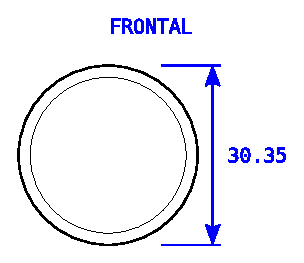
\includegraphics[width=0.25\textwidth]{resources/2.1.circulo.eps}
\caption{Datos del circulo}
\label{circulo}
\end{figure}

\subsection{Calculo del volumen del perno}
\begin{itemize}
\item Dado el perno de la figura \ref{perno}, calcular la formula del
volumen en función de sus parámetros.
\item Calcular el valor del volumen utilizando la formula hallada.
\item Hallar las derivadas parciales de la función con respecto a sus
parámetros.
\item Calcular el error estimado según el criterio pitagórico.
\end{itemize}

\begin{figure}
\centering
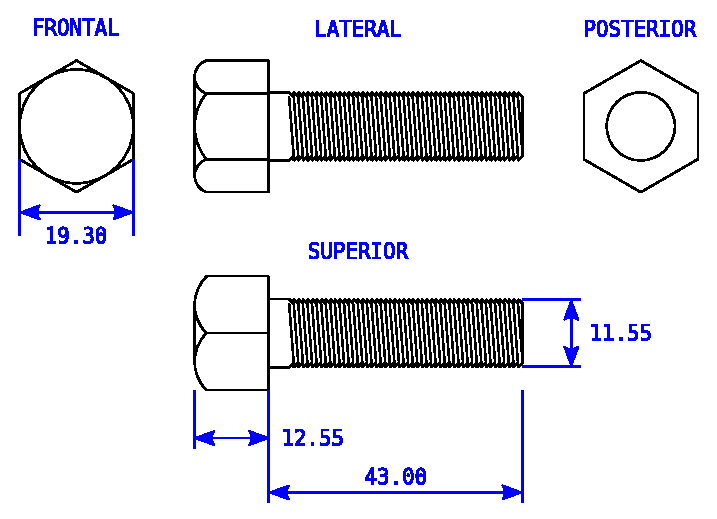
\includegraphics[width=0.58\textwidth]{resources/2.2.perno.eps}
\caption{Datos del perno}
\label{perno}
\end{figure}

\subsection{Calculo del área de la pieza}
\begin{itemize}
\item Dada la pieza de la figura \ref{pieza}, calcular la formula del
área en función de sus parámetros.
\item Calcular el valor del área utilizando la formula hallada.
\item Hallar las derivadas parciales de la función con respecto a sus
parámetros.
\item Calcular el error estimado según el criterio pitagórico.
\end{itemize}

\begin{figure}
\centering
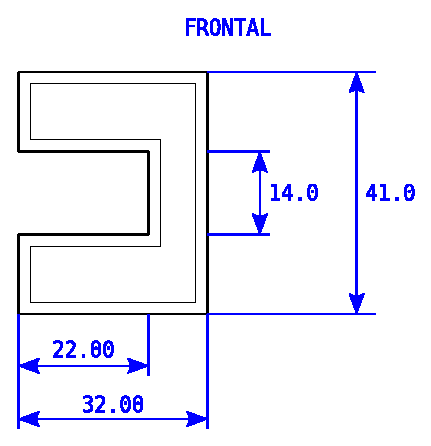
\includegraphics[width=0.35\textwidth]{resources/2.3.pieza.eps}
\caption{Datos de la pieza}
\label{pieza}
\end{figure}

\subsection{Calculo del área de la caja}
\begin{itemize}
\item Dada la caja de la figura \ref{caja}, calcular la formula del
área en función de su base y su altura.
\item Calcular el valor del área utilizando la formula hallada.
\item Hallar las derivadas parciales de la función con respecto a sus
parámetros.
\item Calcular el error estimado según el criterio pitagórico.
\end{itemize}

\begin{figure}
\centering
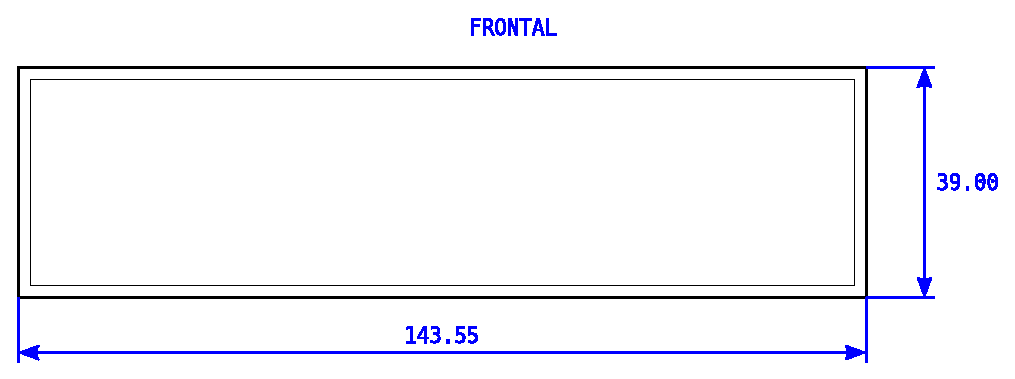
\includegraphics[width=0.85\textwidth]{resources/2.4.caja.eps}
\caption{Datos de la caja}
\label{caja}
\end{figure}

\subsection{Calculo del volumen del capacitor}
\begin{itemize}
\item Dado el capacitor de la figura \ref{capacitor}, calcular la formula del
volumen en función de sus parámetros.
\item Calcular el valor del volumen utilizando la formula hallada.
\item Hallar las derivadas parciales de la función con respecto a sus
parámetros.
\item Calcular el error estimado según el criterio pitagórico.
\end{itemize}

\begin{figure}
\centering
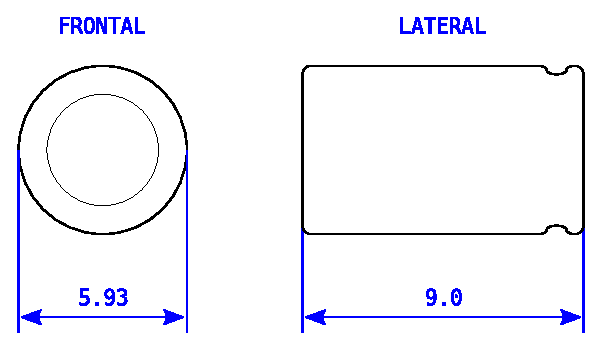
\includegraphics[width=0.53\textwidth]{resources/2.5.capacitor.eps}
\caption{Datos del capacitor}
\label{capacitor}
\end{figure}

\subsection{Calculo del volumen del tornillo}
\begin{itemize}
\item Dado el tornillo de la figura \ref{tornillo}, calcular la formula del
volumen en función de sus parámetros.
\item Calcular el valor del volumen utilizando la formula hallada.
\item Hallar las derivadas parciales de la función con respecto a sus
parámetros.
\item Calcular el error estimado según el criterio pitagórico.
\end{itemize}

\begin{figure}
\centering
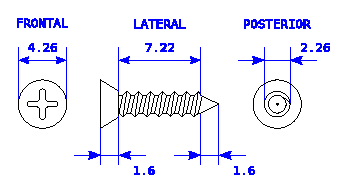
\includegraphics[width=0.52\textwidth]{resources/2.6.tornillo.eps}
\caption{Datos del tornillo}
\label{tornillo}
\end{figure}

\subsection{Calculo del volumen de la esfera}
\begin{itemize}
\item Dada la esfera de la figura \ref{esfera}, calcular la formula del
volumen en función de su diámetro.
\item Calcular el valor del volumen utilizando la formula hallada.
\item Hallar la derivada parcial de la función con respecto a su diámetro.
\item Calcular el error estimado según el criterio pitagórico.
\end{itemize}

\begin{figure}
\centering
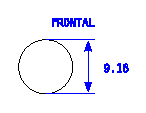
\includegraphics[width=0.20\textwidth]{resources/2.7.esfera.eps}
\caption{Datos de la esfera}
\label{esfera}
\end{figure}

\subsection{Calculo del volumen de la chapa de puerta}
\begin{itemize}
\item Dada la chapa de puerta que se muestra en la imagen \ref{fotografia},
cuyas medidas se presentan en la figura \ref{chapa}, calcular la formula del
volumen en función de sus parámetros.
\item Calcular el valor del volumen utilizando la formula hallada.
\item Hallar las derivadas parciales de la función con respecto a sus
parámetros.
\item Calcular el error estimado según el criterio pitagórico.
\end{itemize}

\begin{figure}
\centering
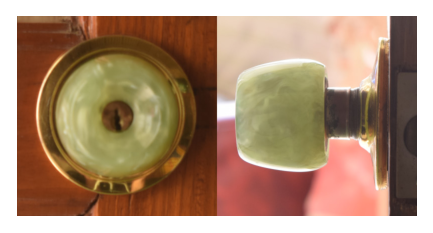
\includegraphics[width=0.80\textwidth]{resources/2.8.chapa1.eps}
\caption{Chapa de puerta a calcular}
\label{fotografia}
\end{figure}

\begin{figure}
\centering
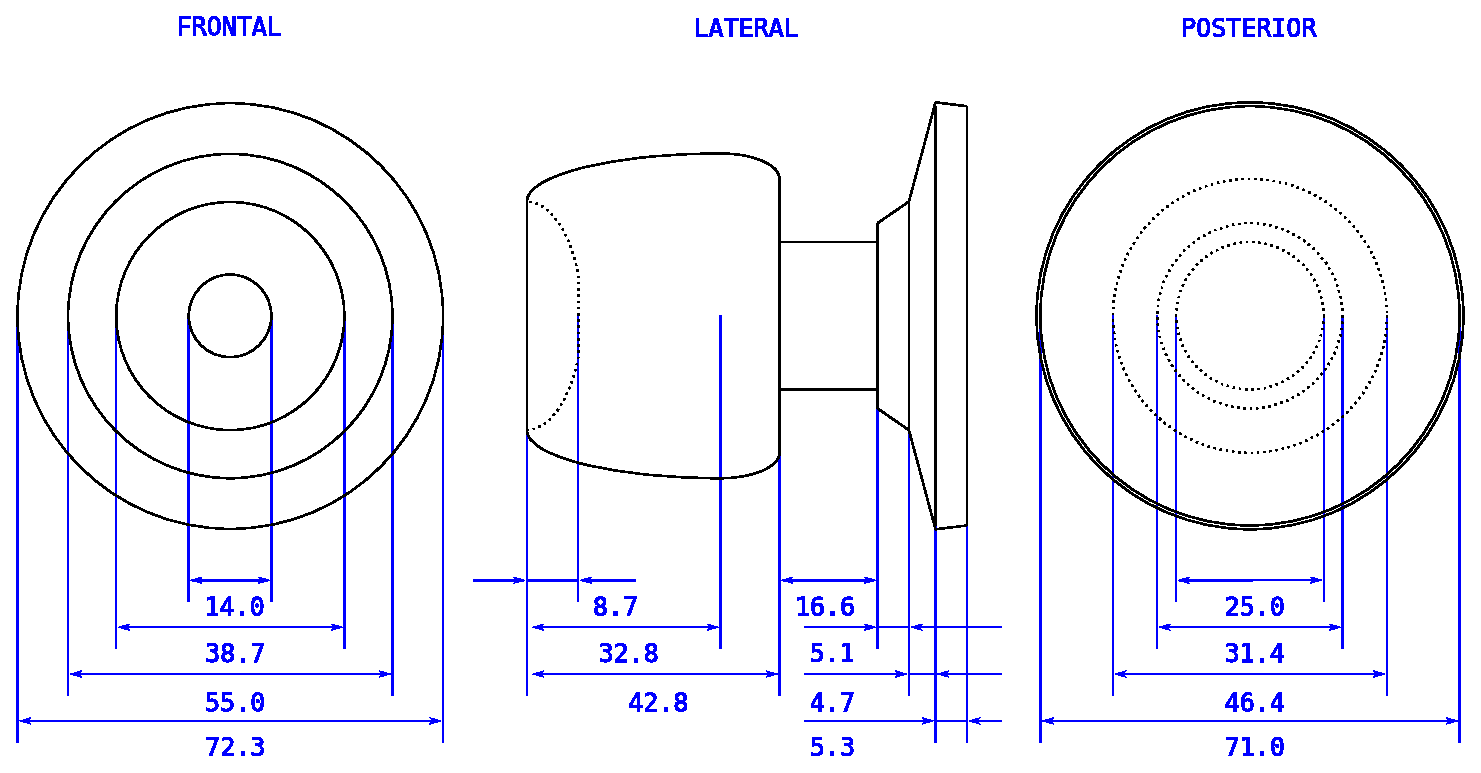
\includegraphics[width=1.00\textwidth]{resources/2.8.chapa2.eps}
\caption{Datos de la chapa}
\label{chapa}
\end{figure}

\section{Tablas de datos y resultados}

\subsection{Calculo del área del circulo}
\vspace*{0.25cm}
\begin{center}
\begin{tabular}{|c|>{\centering}m{5.0cm}<{\centering}|}
\hline
\multicolumn{2}{|c|}{\textbf{Medidas directas del circulo}}
\tabularnewline \hline
Diámetro ($d$) & $30.35 \pm 0.05 [mm]; 0.16\%$ \tabularnewline \hline
\end{tabular}
\end{center}

Dada la ecuación para el calculo del área de un circulo en función de su
diámetro:

\begin{equation}
    A = \pi r^2 = \frac{\pi d^2}{4}
\tag{circulo}
\end{equation}

Calculando el valor representativo:

\begin{equation*}
    A = \frac{(3.1415)(30.35)^2}{4} = 723.45
\end{equation*}

La derivada parcial es:

\begin{equation}
    \frac{\partial{A}}{\partial{d}} = \frac{\pi d}{2}
\end{equation}

Siendo el error de la medición:

\begin{equation}
    e_A = \frac{\pi d}{2} e_d
\end{equation}

Calculando el error representativo:

\begin{equation*}
    e_A = \frac{(3.1415)(30.35)}{2}(0.05) = 2.38
\end{equation*}

\begin{center}
\begin{tabular}{|c|>{\centering}m{5.0cm}<{\centering}|}
\hline
\multicolumn{2}{|c|}{\textbf{Resultado}}
\tabularnewline \hline
Área ($A$) & $723.45 \pm 2.38 [mm^2]; 0.33\%$ \tabularnewline \hline
\end{tabular}
\end{center}

\subsection{Calculo del volumen del perno}
\vspace*{0.25cm}
\begin{center}
\begin{tabular}{|c|>{\centering}m{5.0cm}<{\centering}|}
\hline
\multicolumn{2}{|c|}{\textbf{Medidas directas del perno}}
\tabularnewline \hline
Diámetro de la circunferencia inscrita ($d_i$) & $19.30 \pm 0.05 [mm]; 0.26\%$
\tabularnewline \hline
                 Longitud de la cabeza ($l_h$) & $12.55 \pm 0.05 [mm]; 0.40\%$
\tabularnewline \hline
                  Longitud del vástago ($l_v$) & $43.00 \pm 0.05 [mm]; 0.12\%$
\tabularnewline \hline
                      Diámetro externo ($d_e$) & $11.55 \pm 0.05 [mm]; 0.43\%$
\tabularnewline \hline
\end{tabular}
\end{center}

Dadas las ecuaciones para el calculo del volumen de un prisma hexagonal y un
cilindro, se halla el volumen total del perno:

\begin{equation}
    V_h = 2\sqrt{3} r^2 h = \frac{\sqrt{3}}{2} d^2 h
\tag{prisma}
\end{equation}
\begin{equation}
    V_b = \pi r^2 h = \frac{\pi}{4} d^2 h
\tag{cilindro}
\end{equation}
\begin{equation}
    V = V_h + V_b = \frac{\sqrt{3}}{2} d_i^2 l_h + \frac{\pi}{4} d_e^2 l_v
\end{equation}

Calculando el valor representativo:

\begin{equation*}
    V = \frac{1.7321}{2}(19.30^2)(12.55)+\frac{3.1415}{4}(11.55^2)(43.00)=8553.7
\end{equation*}

Las derivadas parciales son:

\begin{equation}
    \frac{\partial{V}}{\partial{d_i}} = \sqrt{3} d_i l_h
\end{equation}
\begin{equation}
    \frac{\partial{V}}{\partial{l_h}} = \frac{\sqrt{3}}{2} d_i^2
\end{equation}
\begin{equation}
    \frac{\partial{V}}{\partial{d_e}} = \frac{\pi}{2} d_e l_v
\end{equation}
\begin{equation}
    \frac{\partial{V}}{\partial{l_v}} = \frac{\pi}{4} d_e^2
\end{equation}

Siendo el error de la medición:

\begin{equation}
    e_V = \sqrt{
        \left(\sqrt{3}d_il_h\right)^2{e_{di}}^2+
        \left(\frac{\sqrt{3}}{2}d_i^2\right)^2{e_{lc}}^2+
        \left(\frac{\pi}{2}d_el_v\right)^2{e_{de}}^2+
        \left(\frac{\pi}{4}d_e^2\right)^2{e_{lv}}^2
    }
\end{equation}

Calculando el error representativo:

\begin{equation*}
\begin{split}
    e_V^2 = 
        \left((1.7321)(19.30)(12.55)\right)^2(0.05^2)+
        \left(\frac{1.7321}{2}(19.30)^2\right)^2(0.05^2)\\
        +\left(\frac{3.1415}{2}(11.55)(43.00)\right)^2(0.05^2)+
        \left(\frac{3.1415}{4}(11.55)^2\right)^2(0.05^2)
\end{split}
\end{equation*}
\begin{equation*}
    e_V^2 = 440.01 + 260.15 + 1521.5 + 27.444 = 2249.1 
\end{equation*}
\begin{equation*}
    e_V = 47.425
\end{equation*}

\begin{center}
\begin{tabular}{|c|>{\centering}m{5.0cm}<{\centering}|}
\hline
\multicolumn{2}{|c|}{\textbf{Resultado}}
\tabularnewline \hline
Volumen ($V$) & $8553.7 \pm 47.43 [mm^3]; 0.55\%$ \tabularnewline \hline
\end{tabular}
\end{center}

\subsection{Calculo del área de la pieza}
\vspace*{0.25cm}
\begin{center}
\begin{tabular}{|c|>{\centering}m{5.0cm}<{\centering}|}
\hline
\multicolumn{2}{|c|}{\textbf{Medidas directas de la pieza}}
\tabularnewline \hline
  Base externa ($b_e$) & $32.00 \pm 0.05 [mm]; 0.16\%$ \tabularnewline \hline
  Base interna ($b_i$) & $22.00 \pm 0.05 [mm]; 0.23\%$ \tabularnewline \hline
Altura externa ($h_e$) & $41    \pm 1    [mm]; 2.44\%$ \tabularnewline \hline
Altura interna ($h_i$) & $14    \pm 1    [mm]; 7.14\%$ \tabularnewline \hline
\end{tabular}
\end{center}

Dadas las ecuaciones para el calculo del área de un rectángulo, se halla el
área total de la pieza:

\begin{equation}
    A_r = b h
\tag{rectangulo}
\end{equation}
\begin{equation}
    A = b_e h_e - b_i h_i
\end{equation}

Calculando el valor representativo:

\begin{equation*}
    A = (32.00)(41) - (22.00)(14) = 1004
\end{equation*}

Las derivadas parciales son:

\begin{equation}
    \frac{\partial{A}}{\partial{b_e}} = h_e
\end{equation}
\begin{equation}
    \frac{\partial{A}}{\partial{h_e}} = b_e
\end{equation}
\begin{equation}
    \frac{\partial{A}}{\partial{b_i}} = -h_i
\end{equation}
\begin{equation}
    \frac{\partial{A}}{\partial{h_i}} = -b_i
\end{equation}

Siendo el error de la medición:

\begin{equation}
    e_A = \sqrt{
        \left(h_e\right)^2{e_{be}}^2+
        \left(b_e\right)^2{e_{he}}^2+
        \left(-h_i\right)^2{e_{bi}}^2+
        \left(-b_i\right)^2{e_{hi}}^2
    }
\end{equation}

Calculando el error representativo:

\begin{equation*}
    e_A = \sqrt{
        \left(41\right)^2(0.05)^2+
        \left(32.0\right)^2(1)^2+
        \left(-14\right)^2(0.05)^2+
        \left(-22.0\right)^2(1)^2
    }
\end{equation*}
\begin{equation*}
    e_A = \sqrt{4.2025+1024+0.4900+484}
\end{equation*}
\begin{equation*}
    e_A = 38.893
\end{equation*}

\begin{center}
\begin{tabular}{|c|>{\centering}m{5.0cm}<{\centering}|}
\hline
\multicolumn{2}{|c|}{\textbf{Resultado}}
\tabularnewline \hline
Área ($A$) & $1004\pm38.89 [mm^2]; 3.87\%$ \tabularnewline \hline
\end{tabular}
\end{center}

\subsection{Calculo del área de la caja}
\vspace*{0.25cm}
\begin{center}
\begin{tabular}{|c|>{\centering}m{5.0cm}<{\centering}|}
\hline
\multicolumn{2}{|c|}{\textbf{Medidas directas de la caja}}
\tabularnewline \hline
  Base ($b$) & $143.55 \pm 0.05 [mm]; 0.03\%$ \tabularnewline \hline
Altura ($h$) & $ 39    \pm 1    [mm]; 2.56\%$ \tabularnewline \hline
\end{tabular}
\end{center}

Dadas las ecuaciones para el calculo del área de un rectángulo, se halla el
área total de la caja:

\begin{equation}
    A = b h
\tag{rectangulo}
\end{equation}

Calculando el valor representativo:

\begin{equation*}
    A = (143.55)(39) = 5598.5
\end{equation*}

Las derivadas parciales son:

\begin{equation}
    \frac{\partial{A}}{\partial{b}} = h
\end{equation}
\begin{equation}
    \frac{\partial{A}}{\partial{h}} = b
\end{equation}

Siendo el error de la medición:

\begin{equation}
    e_A = \sqrt{
        \left(h\right)^2{e_{b}}^2+
        \left(b\right)^2{e_{h}}^2
    }
\end{equation}

Calculando el error representativo:

\begin{equation*}
    e_A = \sqrt{
        \left(39\right)^2(0.05)^2+
        \left(143.55\right)^2(1)^2
    }
\end{equation*}
\begin{equation*}
    e_A = \sqrt{3.8025+20610.4050}
\end{equation*}
\begin{equation*}
    e_A = 143.56
\end{equation*}

\begin{center}
\begin{tabular}{|c|>{\centering}m{5.0cm}<{\centering}|}
\hline
\multicolumn{2}{|c|}{\textbf{Resultado}}
\tabularnewline \hline
Área ($A$) & $5598.5\pm143.56[mm^2]; 2.56\%$ \tabularnewline \hline
\end{tabular}
\end{center}

\subsection{Calculo del volumen del capacitor}
\vspace*{0.25cm}
\begin{center}
\begin{tabular}{|c|>{\centering}m{5.0cm}<{\centering}|}
\hline
\multicolumn{2}{|c|}{\textbf{Medidas directas del capacitor}}
\tabularnewline \hline
Diámetro ($d$) & $5.93 \pm 0.01 [mm];  0.17\%$ \tabularnewline \hline
  Altura ($h$) & $9    \pm 1    [mm]; 11.11\%$ \tabularnewline \hline
\end{tabular}
\end{center}

Dada la ecuación para el calculo del volumen de un cilindro en función de su
altura y el diámetro de su base:

\begin{equation}
    V = \pi r^2 h = \frac{\pi}{4} d^2 h
\tag{cilindro}
\end{equation}

Calculando el valor representativo:

\begin{equation*}
    V = \frac{(3.1415)(5.93)^2(9)}{4} = 248.57
\end{equation*}

Las derivadas parciales son:

\begin{equation}
    \frac{\partial{V}}{\partial{d}} = \frac{\pi d h}{2}
\end{equation}
\begin{equation}
    \frac{\partial{V}}{\partial{h}} = \frac{\pi d^2}{4}
\end{equation}

Siendo el error de la medición:

\begin{equation}
    e_V = \sqrt{
        \left(\frac{\pi h d}{2}\right)^2{e_d}^2+
        \left(\frac{\pi d^2}{4}\right)^2{e_h}^2
    }
\end{equation}

Calculando el error representativo:

\begin{equation*}
    e_V = \sqrt{
        \left(\frac{(3.1415)(9)(5.93)}{2}\right)^2{0.01}^2+
        \left(\frac{(3.1415)(5.93)^2}{4}\right)^2{1}^2
    }
\end{equation*}
\begin{equation*}
    e_A = \sqrt{0.7028+762.78}
\end{equation*}
\begin{equation*}
    e_A = 27.631
\end{equation*}

\begin{center}
\begin{tabular}{|c|>{\centering}m{5.0cm}<{\centering}|}
\hline
\multicolumn{2}{|c|}{\textbf{Resultado}}
\tabularnewline \hline
Volumen ($V$) & $248.57\pm27.63 [mm^3]; 11.12\%$ \tabularnewline \hline
\end{tabular}
\end{center}

\subsection{Calculo del volumen del tornillo}
\vspace*{0.25cm}
\begin{center}
\begin{tabular}{|c|>{\centering}m{5.0cm}<{\centering}|}
\hline
\multicolumn{2}{|c|}{\textbf{Medidas directas del tornillo}}
\tabularnewline \hline
Diámetro de la cabeza ($d_h$) & $4.26 \pm 0.01 [mm]; 0.23\%$
\tabularnewline \hline
Longitud de la cabeza ($l_h$) & $1.60 \pm 0.01 [mm]; 0.62\%$
\tabularnewline \hline
  Longitud del cuerpo ($l_b$) & $7.22 \pm 0.01 [mm]; 0.14\%$
\tabularnewline \hline
 Longitud de la punta ($l_t$) & $1.60 \pm 0.01 [mm]; 0.62\%$
\tabularnewline \hline
     Diámetro externo ($d_e$) & $2.26 \pm 0.01 [mm]; 0.44\%$
\tabularnewline \hline
\end{tabular}
\end{center}

Dadas las ecuaciones para el calculo del volumen de un cono truncado, cilindro,
y cono, se halla el volumen total del tornillo:

\begin{equation}
    V_1 = \frac{\pi}{3} h (R^2+r^2+Rr) = \frac{\pi}{12} h (D^2+d^2+Dd)
\tag{cono truncado}
\end{equation}
\begin{equation}
    V_2 = \pi r^2 h = \frac{\pi}{4} d^2 h
\tag{cilindro}
\end{equation}
\begin{equation}
    V_3 = \frac{\pi}{3} r^2 h = \frac{\pi}{12} d^2 h
\tag{cono}
\end{equation}
\begin{equation}
    V = V_1 + V_2 + V_3 = \frac{\pi}{12} l_h (d_h^2+d_e^2+d_h d_e) +
    \frac{\pi}{4} d_e l_b + \frac{\pi}{12} d_e l_t
\end{equation}

Calculando el valor representativo:

\begin{equation*}
\begin{split}
    V = \frac{3.1415}{12}(1.60)(4.25^2+2.26^2+(4.26)(2.26))\\
    +\frac{3.1415}{4}(2.26)(7.22)+\frac{3.1415}{12}(2.26)(1.60)
\end{split}
\end{equation*}
\begin{equation*}
    V = 13.774 + 12.815 + 0.9467 = 27.536
\end{equation*}

Las derivadas parciales son:

\begin{equation}
    \frac{\partial{V}}{\partial{l_h}}=\frac{\pi}{12}(d_h^2+d_e^2+d_h d_e)
\end{equation}
\begin{equation}
    \frac{\partial{V}}{\partial{d_h}}=\frac{\pi}{6}l_h(d_h+\frac{d_e}{2})
\end{equation}
\begin{equation}
    \frac{\partial{V}}{\partial{d_e}}=\frac{\pi}{6}l_h(d_e+\frac{d_h}{2})
    +\frac{\pi}{4}l_b+\frac{\pi}{12}l_t
\end{equation}
\begin{equation}
    \frac{\partial{V}}{\partial{l_b}} = \frac{\pi}{4} d_e
\end{equation}
\begin{equation}
    \frac{\partial{V}}{\partial{l_t}} = \frac{\pi}{12} d_e
\end{equation}

Siendo el error de la medición:

\begin{equation}
\begin{split}
    e_V^2 = 
        \left(\frac{\pi}{12}(d_h^2+d_e^2+d_h d_e)\right)^2{e_{lh}}^2
        +\left(\frac{\pi}{6}l_h(d_h+\frac{d_e}{2})\right)^2{e_{dh}}^2 \\
        +\left(\frac{\pi}{6}l_h(d_e+\frac{d_h}{2})+\frac{\pi}{4}l_b
        +\frac{\pi}{12}l_t\right)^2{e_{de}}^2 \\
        +\left(\frac{\pi}{4} d_e\right)^2{e_{lb}}^2
        +\left(\frac{\pi}{12} d_e\right)^2{e_{lt}}^2
\end{split}
\end{equation}

Calculando el error representativo:

\begin{equation*}
\begin{split}
    e_V^2 = 
        \left(\frac{3.1415}{12}((4.26)^2+(2.26)^2
        +(4.26)(2.26))\right)^2 0.01^2 \\
        +\left(\frac{3.1415}{6}(1.60)((4.26)+\frac{2.26}{2})\right)^2 0.01^2 \\
        +\left(\frac{3.1415}{6}(1.60)(2.26+\frac{4.26}{2})
        +\frac{3.1415}{4}(7.22)
        +\frac{3.1415}{12}(1.60)\right)^2 0.01^2 \\
        +\left(\frac{3.1415}{4}(2.26)\right)^2 0.01^2
        +\left(\frac{3.1415}{12}(2.26)\right)^2 0.01^2
\end{split}
\end{equation*}
\begin{equation*}
    e_V^2 = 0.007+0.002+0.009+0.0003+0.00003 = 0.0193
\end{equation*}
\begin{equation*}
    e_V = 0.14
\end{equation*}

\begin{center}
\begin{tabular}{|c|>{\centering}m{5.0cm}<{\centering}|}
\hline
\multicolumn{2}{|c|}{\textbf{Resultado}}
\tabularnewline \hline
Volumen ($V$) & $27.54\pm0.14 [mm^3]; 0.50\%$ \tabularnewline \hline
\end{tabular}
\end{center}

\subsection{Calculo del volumen de la esfera}
\vspace*{0.25cm}
\begin{center}
\begin{tabular}{|c|>{\centering}m{5.0cm}<{\centering}|}
\hline
\multicolumn{2}{|c|}{\textbf{Medidas directas de la esfera}}
\tabularnewline \hline
Diámetro de la esfera ($d$) & $9.16 \pm 0.01 [mm]; 0.11\%$
\tabularnewline \hline
\end{tabular}
\end{center}

Dada la ecuación para el calculo del volumen de la esfera en función de su
diámetro:

\begin{equation}
    V = \frac{4}{3} \pi r^3 = \frac{\pi d^3}{6}
\tag{esfera}
\end{equation}

Calculando el valor representativo:

\begin{equation*}
    V = \frac{3.1415}{6} 9.16^3 = 402.43
\end{equation*}

La derivada parcial es:

\begin{equation}
    \frac{\partial{V}}{\partial{d}} = \frac{\pi}{2} d^2
\end{equation}

Siendo el error de la medición:

\begin{equation}
    e_V = \frac{\pi}{2} d^2 e_d
\end{equation}

Calculando el error representativo:

\begin{equation*}
    e_V = \frac{3.1415}{2}(9.16)^2(0.01) = 1.3180
\end{equation*}

\begin{center}
\begin{tabular}{|c|>{\centering}m{5.0cm}<{\centering}|}
\hline
\multicolumn{2}{|c|}{\textbf{Resultado}}
\tabularnewline \hline
Volumen ($V$) & $402.43 \pm 1.32 [mm^3]; 0.33\%$ \tabularnewline \hline
\end{tabular}
\end{center}

\subsection{Calculo del volumen de la chapa de puerta}
\vspace*{0.25cm}
\begin{center}
\begin{tabular}{|c|>{\centering}m{5.0cm}<{\centering}|}
\hline
\multicolumn{2}{|c|}{\textbf{Medidas directas de la chapa}}
\tabularnewline \hline
         Diámetro cilindro ($d_1$) & $14.0 \pm 0.1 [mm]; 0.71\%$
\tabularnewline \hline
      Diámetro mínimo pomo ($d_2$) & $38.7 \pm 0.1 [mm]; 0.26\%$
\tabularnewline \hline
      Diámetro máximo pomo ($d_3$) & $55.0 \pm 0.1 [mm]; 0.18\%$
\tabularnewline \hline
    Diámetro máximo roseta ($d_4$) & $72.3 \pm 0.1 [mm]; 0.14\%$
\tabularnewline \hline
           Diámetro cuello ($d_5$) & $25.0 \pm 0.1 [mm]; 0.40\%$
\tabularnewline \hline
    Diámetro mínimo roseta ($d_6$) & $31.4 \pm 0.1 [mm]; 0.32\%$
\tabularnewline \hline
Diámetro intermedio roseta ($d_7$) & $46.4 \pm 0.1 [mm]; 0.22\%$
\tabularnewline \hline
     Diámetro borde roseta ($d_8$) & $71.0 \pm 0.1 [mm]; 0.14\%$
\tabularnewline \hline
          Profundidad pomo ($l_1$) & $ 8.7 \pm 0.1 [mm]; 1.15\%$
\tabularnewline \hline
     Longitud barriga pomo ($l_2$) & $32.8 \pm 0.1 [mm]; 0.30\%$
\tabularnewline \hline
             Longitud pomo ($l_3$) & $42.8 \pm 0.1 [mm]; 0.23\%$
\tabularnewline \hline
           Longitud cuello ($l_4$) & $16.6 \pm 0.1 [mm]; 0.60\%$
\tabularnewline \hline
      Grosor cuello roseta ($l_5$) & $ 5.1 \pm 0.1 [mm]; 1.96\%$
\tabularnewline \hline
  Grosor intermedio roseta ($l_6$) & $ 4.7 \pm 0.1 [mm]; 2.13\%$
\tabularnewline \hline
        Grosor base roseta ($l_7$) & $ 5.3 \pm 0.1 [mm]; 1.89\%$
\tabularnewline \hline
\end{tabular}
\end{center}

Dadas las ecuaciones para el calculo del volumen de un cono truncado, un
cilindro, y un tonel; se halla el volumen total de la chapa:

\begin{equation}
    V_a(h,D,d) = \frac{\pi}{12} h (D^2+d^2+Dd)
\tag{cono truncado}
\end{equation}
\begin{equation}
    V_b(h,d) = \frac{\pi}{4} h d^2
\tag{cilindro}
\end{equation}
\begin{equation}
    V_c(h,D,d) = \frac{\pi}{12} h (2D^2-d^2)
\tag{tonel}
\end{equation}
\begin{equation*}
\begin{split}
    V=V_a(l_7,d_4,d_8)+V_a(l_6,d_4,d_2)+V_a(l_5,d_2,d_6)+V_b(l_4,d_5) \\
    +\frac{V_c(2(l_3-l_2),d_3,d_7)}{2}
    +\frac{V_c(2 l_2,d_3,d_2)}{2}
    -\frac{V_c(2 l_1,d_2,d_1)}{2}
\end{split}
\end{equation*}
\begin{equation*}
\begin{split}
    V=\frac{\pi}{12}l_7(d_4^2+d_4 d_8+d_8^2)
     +\frac{\pi}{12}l_6(d_4^2+d_4 d_2+d_2^2)
     +\frac{\pi}{12}l_5(d_2^2+d_2 d_6+d_6^2)
     +\frac{\pi}{4}l_4 d_5^2 \\
     +\frac{\pi}{12}(2l_3 d_3^2+l_3 d_7^2-2 l_2 d_3^2+l_2 d_7^2)
     +\frac{\pi}{6}l_2(2d_3^2-d_2^2)
     -\frac{\pi}{6}l_1(2d_2^2-d_1^2)
\end{split}
\end{equation*}
\begin{equation}
\begin{split}
    V=\frac{\pi}{12}l_7 d_4^2+\frac{\pi}{12}l_7 d_4 d_8
     +\frac{\pi}{12}l_7 d_8^2 \\
     +\frac{\pi}{12}l_6 d_4^2+\frac{\pi}{12}l_6 d_4 d_2
     +\frac{\pi}{12}l_6 d_2^2 \\
     +\frac{\pi}{12}l_5 d_2^2+\frac{\pi}{12}l_5 d_2 d_6
     +\frac{\pi}{12}l_5 d_6^2 \\
     +\frac{\pi}{4}l_4 d_5^2 \\
     +\frac{\pi}{6}l_3 d_3^2+\frac{\pi}{12}l_3 d_7^2 \\
     +\frac{\pi}{6}l_2 d_3^2+\frac{\pi}{12}l_2 d_7^2-\frac{\pi}{3}l_2 d_2^2 \\
     -\frac{\pi}{3}l_1 d_2^2+\frac{\pi}{6}l_1 d_1^2
\end{split}
\end{equation}

Calculando el valor representativo:

\begin{equation*}
\begin{split}
    V=\frac{3.1415}{12}(5.3)(72.3)^2+\frac{3.1415}{12}(5.3)(72.3)(71)
     +\frac{3.1415}{12}(5.3)(71)^2 \\
     +\frac{3.1415}{12}(4.7)(72.3)^2+\frac{3.1415}{12}(4.7)(72.3)(38.7)
     +\frac{3.1415}{12}(4.7)(38.7)^2 \\
     +\frac{3.1415}{12}(5.1)(38.7)^2+\frac{3.1415}{12}(5.1)(38.7)(31.4)
     +\frac{3.1415}{12}(5.1)(31.4)^2 \\
     +\frac{3.1415}{4}(16.6)(25)^2 \\
     +\frac{3.1415}{6}(42.8)(55)^2+\frac{3.1415}{12}(42.8)(46.4)^2 \\
     +\frac{3.1415}{6}(32.8)(55)^2+\frac{3.1415}{12}(32.8)(46.4)^2
     -\frac{3.1415}{3}(32.8)(38.7)^2 \\
     -\frac{3.1415}{3}(8.7)(38.7)^2+\frac{3.1415}{6}(8.7)(14)^2
\end{split}
\end{equation*}
\begin{equation*}
    V = 21370.27+11717.63+4938.60+8148.5+91914.28+18996.20-12752.04
\end{equation*}
\begin{equation*}
    V = 144333.44
\end{equation*}

Las derivadas parciales son:

\begin{equation}
    \frac{\partial{V}}{\partial{d_1}}=\frac{\pi}{3}l_1 d_1
\end{equation}
\begin{equation}
    \frac{\partial{V}}{\partial{d_2}}=\frac{\pi}{12}l_6 d_4
    +\frac{\pi}{6}l_6 d_2+\frac{\pi}{6}l_5 d_2+\frac{\pi}{12}l_5 d_6
    -\frac{2\pi}{3}l_2 d_2-\frac{2\pi}{3}l_1 d_2
\end{equation}
\begin{equation}
    \frac{\partial{V}}{\partial{d_3}}=\frac{\pi}{3}l_3 d_3+\frac{\pi}{3}l_2 d_3
\end{equation}
\begin{equation}
    \frac{\partial{V}}{\partial{d_4}}=\frac{\pi}{6}l_7 d_4
    +\frac{\pi}{12}l_7 d_8+\frac{\pi}{6}l_6 d_4+\frac{\pi}{12}l_6 d_2
\end{equation}
\begin{equation}
    \frac{\partial{V}}{\partial{d_5}}=\frac{\pi}{2}l_4 d_5
\end{equation}
\begin{equation}
    \frac{\partial{V}}{\partial{d_6}}=\frac{\pi}{12}l_5 d_2+\frac{\pi}{6}l_5 d_6
\end{equation}
\begin{equation}
    \frac{\partial{V}}{\partial{d_7}}=\frac{\pi}{6}l_3 d_7+\frac{\pi}{6}l_2 d_7
\end{equation}
\begin{equation}
    \frac{\partial{V}}{\partial{d_8}}=\frac{\pi}{12}l_7 d_4+\frac{\pi}{6}l_7 d_8
\end{equation}
\begin{equation}
    \frac{\partial{V}}{\partial{l_1}}=-\frac{\pi}{3}d_2^2+\frac{\pi}{6}d_1^2
\end{equation}
\begin{equation}
    \frac{\partial{V}}{\partial{l_2}}=\frac{\pi}{6}d_3^2+\frac{\pi}{12}d_7^2
    -\frac{\pi}{3}d_2^2
\end{equation}
\begin{equation}
    \frac{\partial{V}}{\partial{l_3}}=\frac{\pi}{6}d_3^2+\frac{\pi}{12}d_7^2
\end{equation}
\begin{equation}
    \frac{\partial{V}}{\partial{l_4}}=\frac{\pi}{4}d_5^2
\end{equation}
\begin{equation}
    \frac{\partial{V}}{\partial{l_5}}=\frac{\pi}{12}d_2^2+\frac{\pi}{12}d_2 d_6
    +\frac{\pi}{12}d_6^2
\end{equation}
\begin{equation}
    \frac{\partial{V}}{\partial{l_6}}=\frac{\pi}{12}d_4^2+\frac{\pi}{12}d_4 d_2
    +\frac{\pi}{12}d_2^2
\end{equation}
\begin{equation}
    \frac{\partial{V}}{\partial{l_7}}=\frac{\pi}{12}d_4^2+\frac{\pi}{12}d_4 d_8
    +\frac{\pi}{12}d_8^2
\end{equation}

Siendo el error de la medición:

\begin{equation}
\begin{split}
    e_V^2 = 
         \left(
            \frac{\pi}{3}l_1 d_1
        \right)^2{e_{d1}}^2
        +\left(
             \frac{\pi}{12}l_6 d_4+\frac{\pi}{6}l_6 d_2+\frac{\pi}{6}l_5 d_2
            +\frac{\pi}{12}l_5 d_6-\frac{2\pi}{3}l_2 d_2
            -\frac{2\pi}{3}l_1 d_2
        \right)^2{e_{d2}}^2 \\
        +\left(
            \frac{\pi}{3}l_3 d_3+\frac{\pi}{3}l_2 d_3
        \right)^2{e_{d3}}^2
        +\left(
             \frac{\pi}{6}l_7 d_4+\frac{\pi}{12}l_7 d_8
            +\frac{\pi}{6}l_6 d_4+\frac{\pi}{12}l_6 d_2
        \right)^2{e_{d4}}^2 \\
        +\left(
            \frac{\pi}{2}l_4 d_5
        \right)^2{e_{d5}}^2
        +\left(
            \frac{\pi}{12}l_5 d_2+\frac{\pi}{6}l_5 d_6
        \right)^2{e_{d6}}^2
        +\left(
            \frac{\pi}{6}l_3 d_7+\frac{\pi}{6}l_2 d_7
        \right)^2{e_{d7}}^2 \\
        +\left(
             \frac{\pi}{12}l_7 d_4+\frac{\pi}{6}l_7 d_8
        \right)^2{e_{d8}}^2
        +\left(
            -\frac{\pi}{3}d_2^2+\frac{\pi}{6}d_1^2
        \right)^2{e_{l1}}^2
        +\left(
            \frac{\pi}{6}d_3^2+\frac{\pi}{12}d_7^2-\frac{\pi}{3}d_2^2
        \right)^2{e_{l2}}^2 \\
        +\left(
            \frac{\pi}{6}d_3^2+\frac{\pi}{12}d_7^2
        \right)^2{e_{l3}}^2
        +\left(
            \frac{\pi}{4}d_5^2
        \right)^2{e_{l4}}^2
        +\left(
            \frac{\pi}{12}d_2^2+\frac{\pi}{12}d_2 d_6+\frac{\pi}{12}d_6^2
        \right)^2{e_{l5}}^2 \\
        +\left(
            \frac{\pi}{12}d_4^2+\frac{\pi}{12}d_4 d_2+\frac{\pi}{12}d_2^2
        \right)^2{e_{l6}}^2
        +\left(
            \frac{\pi}{12}d_4^2+\frac{\pi}{12}d_4 d_8+\frac{\pi}{12}d_8^2
        \right)^2{e_{l7}}^2
\end{split}
\end{equation}

Calculando el error representativo:

\begin{equation*}
\begin{split}
    e_V^2 = 
         \Biggl(
            \frac{3.1415}{3}(8.7)(14)
        \Biggr)^2{0.1}^2
        +\Biggl(
             \frac{3.1415}{12}(4.7)(72.3)
            +\frac{3.1415}{6}(4.7)(38.7)
            +\frac{3.1415}{6}(5.1)(38.7) \\
            +\frac{3.1415}{12}(5.1)(31.4)
            -\frac{2(3.1415)}{3}(32.8)(38.7)
            -\frac{2(3.1415)}{3}(8.7)(38.7)
        \Biggr)^2{0.1}^2 \\
        +\Biggl(
             \frac{3.1415}{3}(42.8)(55)
            +\frac{3.1415}{3}(32.8)(55)
        \Biggr)^2{0.1}^2
        +\Biggl(
             \frac{3.1415}{6}(5.3)(72.3)+\frac{3.1415}{12}(5.3)(71) \\
            +\frac{3.1415}{6}(4.7)(72.3)+\frac{3.1415}{12}(4.7)(38.7)
        \Biggr)^2{0.1}^2
        +\Biggl(
            \frac{3.1415}{2}(16.6)(25)
        \Biggr)^2{0.1}^2 \\
        +\Biggl(
             \frac{3.1415}{12}(5.1)(38.7)
            +\frac{3.1415}{6}(5.1)(31.4)
        \Biggr)^2{0.1}^2
        +\Biggl(
             \frac{3.1415}{6}(42.8)(46.4) \\
            +\frac{3.1415}{6}(32.8)(46.4)
        \Biggr)^2{0.1}^2
        +\Biggl(
             \frac{3.1415}{12}(5.3)(72.3)+\frac{3.1415}{6}(5.3)(71)
        \Biggr)^2{0.1}^2 \\
        +\Biggl(
            -\frac{3.1415}{3}(38.7)^2
            +\frac{3.1415}{6}(14)^2
        \Biggr)^2{0.1}^2
        +\Biggl(
            \frac{3.1415}{6}(55)^2+\frac{3.1415}{12}(46.4)^2-\frac{3.1415}{3}(38.7)^2
        \Biggr)^2{0.1}^2 \\
        +\Biggl(
            \frac{3.1415}{6}(55)^2+\frac{3.1415}{12}(46.4)^2
        \Biggr)^2{0.1}^2
        +\Biggl(
            \frac{3.1415}{4}(25)^2
        \Biggr)^2{0.1}^2
        +\Biggl(
             \frac{3.1415}{12}(38.7)^2 \\
            +\frac{3.1415}{12}(38.7)(31.4)
            +\frac{3.1415}{12}(31.4)^2
        \Biggr)^2{0.1}^2
        +\Biggl(
             \frac{3.1415}{12}(72.3)^2
            +\frac{3.1415}{12}(72.3)(38.7) \\
            +\frac{3.1415}{12}(38.7)^2
        \Biggr)^2{0.1}^2
        +\Biggl(
             \frac{3.1415}{12}(72.3)^2
            +\frac{3.1415}{12}(72.3)(71)
            +\frac{3.1415}{12}(71)^2
        \Biggr)^2{0.1}^2
\end{split}
\end{equation*}
\begin{equation*}
\begin{split}
    e_V^2 = (127.55)^2(0.01)+(-3034.2)^2(0.01)+(24075.07)^2(0.01) \\
        +(524.70)^2(0.01)+(651.88)^2(0.01)+(135.52)^2(0.01) \\
        +(1836.7)^2(0.01)+(297.35)^2(0.01)+(-1465.8)^2(0.01) \\
        +(579.15)^2(0.01)+(2147.5)^2(0.01)+(490.87)^2(0.01) \\
        +(968.35)^2(0.01)+(2493.1)^2(0.01)+(4032.1)^2(0.01) 
\end{split}
\end{equation*}
\begin{equation*}
    e_V^2 = 6237604.95
\end{equation*}
\begin{equation*}
    e_V = 2497.5
\end{equation*}

\begin{center}
\begin{tabular}{|c|>{\centering}m{7.0cm}<{\centering}|}
\hline
\multicolumn{2}{|c|}{\textbf{Resultado}}
\tabularnewline \hline
Volumen ($V$) & $144333.44\pm2497.5 [mm^3]; 1.73\%$ \tabularnewline \hline
\end{tabular}
\end{center}

\section{Conclusiones}
Puede notarse que las mediciones indirectas agrandan el error que las mediciones
directas ya tienen, se ha considerado mejorar la precisión de los instrumentos
para objetos que son pequeños.

\subsection{Resumen de mediciones}
A continuación se resumen las medidas obtenidas:

\begin{center}
\begin{tabular}{|c|>{\centering}m{6.0cm}<{\centering}|}
\hline
     \textbf{Área del circulo} & $723.45 \pm 2.38 [mm^2]; 0.33\%$
\tabularnewline \hline
    \textbf{Volumen del perno} & $8553.7 \pm 47.43 [mm^3]; 0.55\%$
\tabularnewline \hline
     \textbf{Área de la pieza} & $1004\pm38.89 [mm^2]; 3.87\%$
\tabularnewline \hline
      \textbf{Área de la caja} & $5598.5\pm143.56[mm^2]; 2.56\%$
\tabularnewline \hline
\textbf{Volumen del capacitor} & $248.57\pm27.63 [mm^3]; 11.12\%$
\tabularnewline \hline
 \textbf{Volumen del tornillo} & $27.54\pm0.14 [mm^3]; 0.50\%$
\tabularnewline \hline
    \textbf{Volumen de esfera} & $402.43 \pm 1.32 [mm^3]; 0.33\%$
\tabularnewline \hline
     \textbf{Volumen de chapa} & $144333.44\pm2497.5 [mm^3]; 1.73\%$
\tabularnewline \hline
\end{tabular}\\
\end{center}

\section{Referencias bibliográficas}
\begin{itemize}
\item Errores de medición y su propagación \\
http://www.tplaboratorioquimico.com/2008/08/errores-de-medicion-y-su-propagacion.html
\item Tratamiento y propagación de errores \\
http://www.lawebdefisica.com/apuntsfis/errores/
\item Informe de propagación de errores \\
http://www.slideshare.net/cdloor/informe-de-propagacion-de-errores-laboratorio-de-fisica-c
\item Guía práctica para la realización de la medida y el calculo de errores \\
http://bacterio.uc3m.es/docencia/laboratorio/guiones\_esp/errores/guiondeerrores.pdf
\end{itemize}

\end{document}
